\section{Load Balancing Scenarios Topology Generator}
In this work, we use random topologies for both data collection to
train the model and for evaluating the performance of the proposed OF.

The topologies are generated in Python and convert into file that
Cooja and read and understand.
The root node sits in the middle of the network and is the server
that receives packets from the clients.
The rest of the nodes are either the client or overloading client,
which transmit data at a higher rate, representing devices that
generate high traffic such as camera.
The clients are added to the network sequentially by taking random
point within the reach of existed nodes in the network. The new node
must be in the
transmission range of other nodes and must be at least a certain
distance from all node. This ensure that the network is connected
while make sure that the nodes are distributed evenly without a hotspot.

Afterward, 5\% of the nodes are selected at random to be the
overloading client that send 30 packets per minute, representing
devices that produce high traffic such as camera or ...

So in all, each topology have a topology seed, which determines the node
placement in the network, and a client seed, which determines which
client nodes are selected as overloading clients.
Figure~\ref{fig:topology-random1} gives an example of a random
topologies with 40 nodes.

\begin{fig}[tbh]
    \begin{center}
        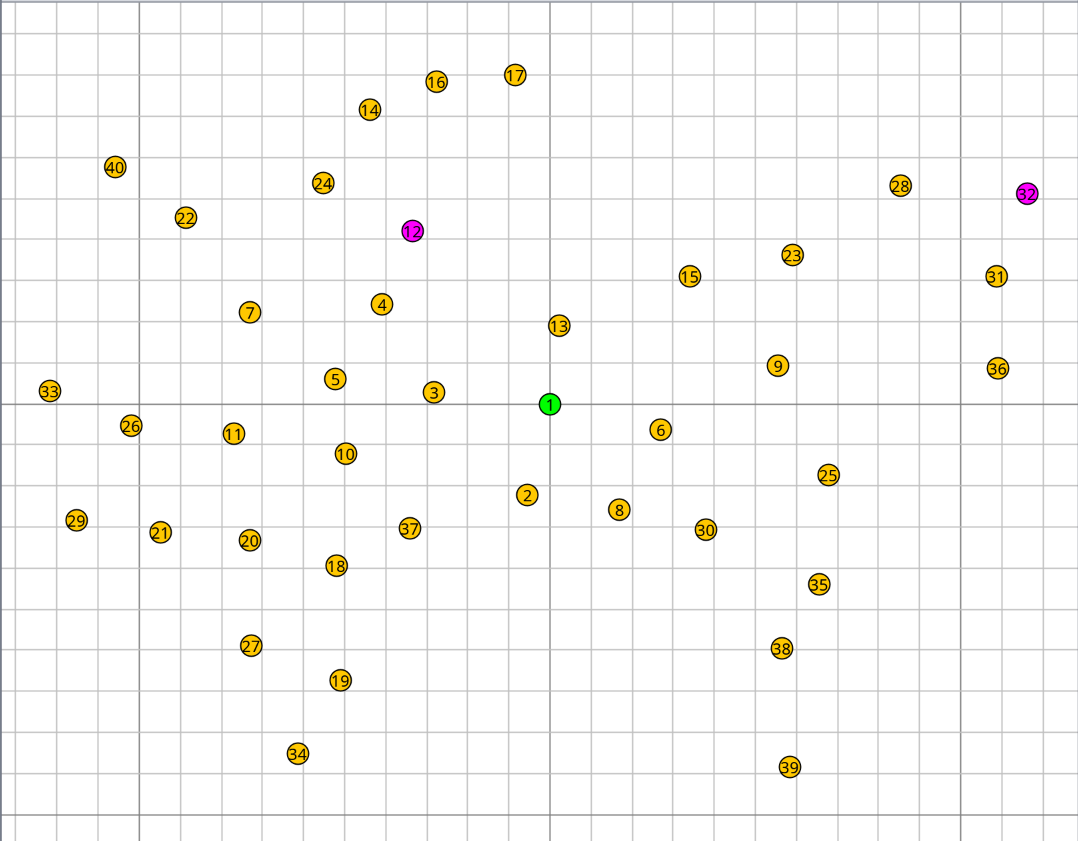
\includegraphics[width=0.7\textwidth]{assets/topology_random1.png}
        \caption{A random generated topology with 40 nodes, the green
            node is the root node, the yellow nodes are normal client and
        the pink nodes are overloading client.}
        \label{fig:topology-random1}
    \end{center}
\end{fig}
